% Provenance (never printed): 6e geography and cycle 3 sciences (locating a
% place on the globe: parallels, meridians, latitude, longitude; the Earth's
% rotation and time zones); see sources/book1/PROVENANCE.md.
% Book 1, grade 6, chapter 2.
\chapter{अक्षांश, देशांतर और समय-क्षेत्र}\label{ch:g6:latitude-longitude}

\omterm{def:g2:water-on-earth:ocean}{महासागर} पर रात उतर आई है। साल 1750 में, एक पाल वाले जहाज़ के डेक पर, नाविक अपना
यंत्र एक चमकीले तारे की ओर उठाता है और नापता है कि वह \omterm{def:g2:water-on-earth:ocean}{समुद्र} से कितना ऊँचा है।
कुछ मिनट का काम, और वह जान जाता है कि जहाज़ \omterm{def:g3:continents-and-oceans:equator}{भूमध्य रेखा} से कितना उत्तर में है। पर
पूर्व या पश्चिम में कितना? यह वह नहीं बता सकता। यह समस्या इतनी गंभीर थी कि 1714
में ब्रिटिश संसद ने उस व्यक्ति के लिए एक बड़े इनाम का वादा किया था जो इसे \omterm{def:g2:water-on-earth:ocean}{समुद्र} में
नापने का तरीक़ा खोज ले। आज तुम्हारी जेब का फ़ोन दोनों जवाब एक सेकंड में देता है।
% ledger: rmg:15deg-per-hour, rmg:longitude-act-1714

\begin{omfigure}
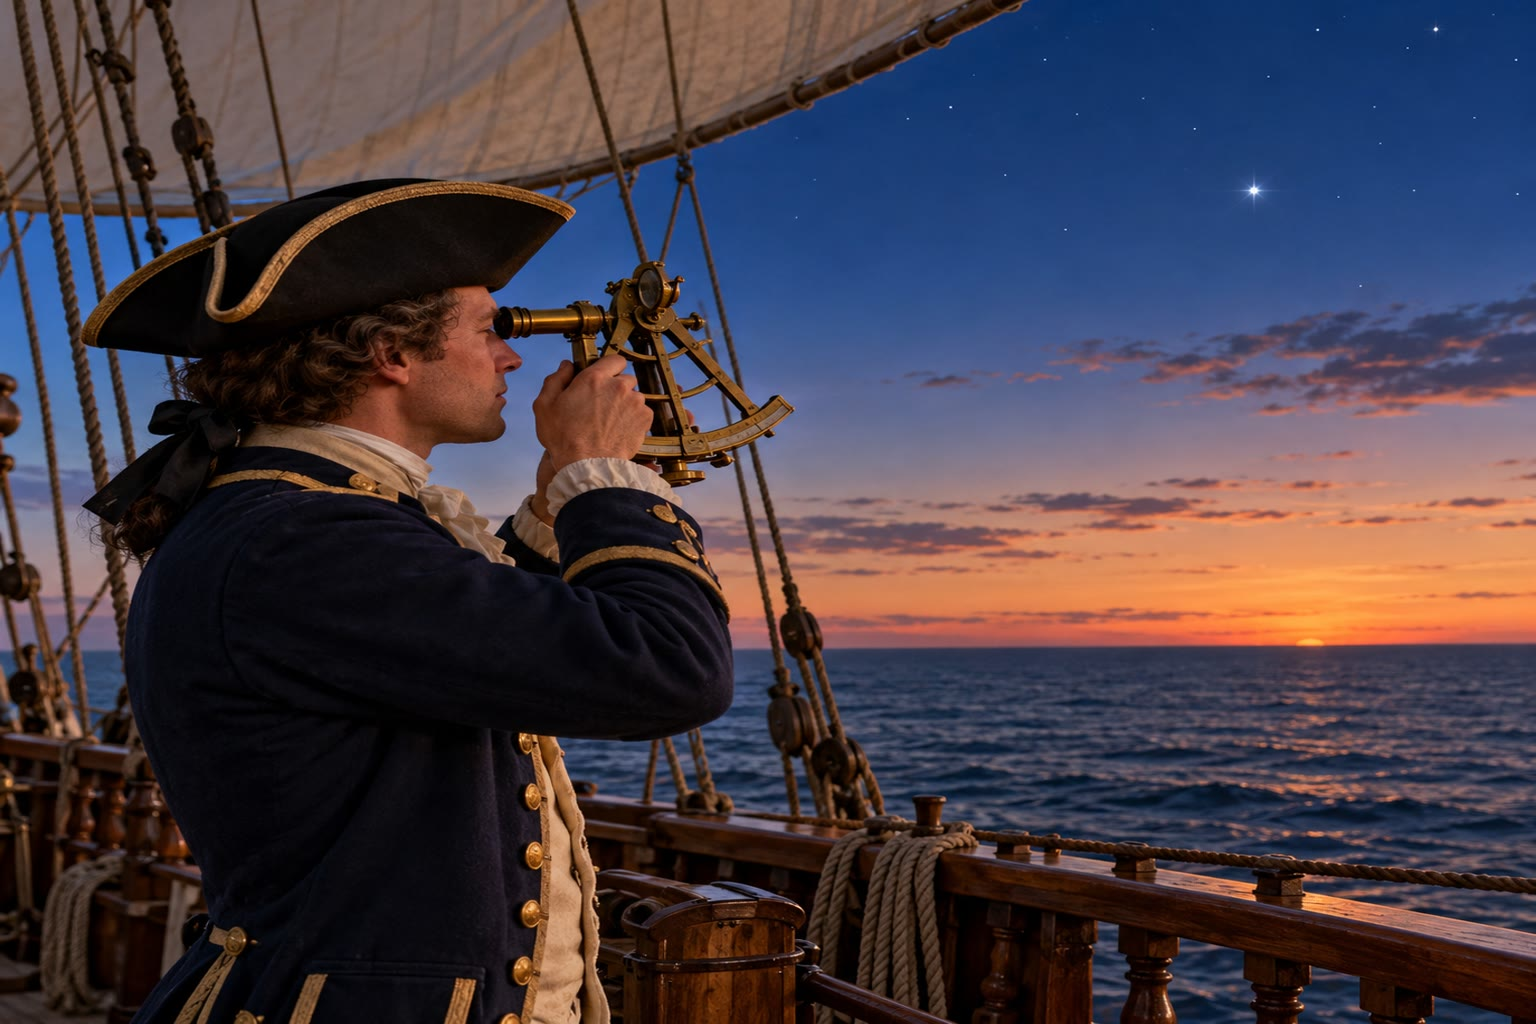
\includegraphics[width=0.62\linewidth]{images/book1/ai/g6-navigator-sextant.jpg}

{\small अठारहवीं सदी का एक नाविक \omterm{def:g2:water-on-earth:ocean}{समुद्र} के क्षितिज के ऊपर एक तारे की ऊँचाई नापता
है। (AI चित्रण।)}
\end{omfigure}

\begin{recall}
\omterm{def:g3:continents-and-oceans:globe}{ग्लोब} पृथ्वी का एक छोटा मॉडल है। \omterm{def:g3:continents-and-oceans:equator}{भूमध्य रेखा} वह रेखा है जो \omterm{def:g3:continents-and-oceans:globe}{ग्लोब} के बीचोंबीच चारों
ओर जाती है, \omterm{def:g3:continents-and-oceans:poles}{उत्तरी ध्रुव} और \omterm{def:g3:continents-and-oceans:poles}{दक्षिणी ध्रुव} के ठीक आधे रास्ते पर; वह पृथ्वी को \omterm{def:g3:continents-and-oceans:equator}{उत्तरी
गोलार्ध} और \omterm{def:g3:continents-and-oceans:equator}{दक्षिणी गोलार्ध} में काटती है (\cref{ch:g3:continents-and-oceans})।
भौतिकी की पुस्तकों ने दिखाया कि पृथ्वी दोनों \omterm{def:g3:continents-and-oceans:poles}{ध्रुवों} से होकर जाने वाले एक अक्ष के
चारों ओर दिन में एक बार अपने-आप पर घूमती है: यह घूमना दिन और रात
लाता है।
\end{recall}

\section{अक्षांश रेखाएँ और अक्षांश}

पृथ्वी पर कोई जगह कहाँ है, यह बताने के लिए हमें दो संख्याएँ चाहिए, सिनेमाघर में
किसी सीट की पंक्ति और स्तंभ की तरह। पहली बताती है कि जगह \omterm{def:g3:continents-and-oceans:equator}{भूमध्य रेखा} से कितना
उत्तर या दक्षिण में है।

कल्पना करो कि पृथ्वी को दोनों \omterm{def:g3:continents-and-oceans:poles}{ध्रुवों} से होकर दो हिस्सों में काटा गया है, जैसे किसी
सेब को डंठल से नीचे की ओर काटते हैं। कटे हुए फलक पर (नीचे, बाईं ओर), \omterm{def:g3:continents-and-oceans:equator}{भूमध्य रेखा}
केंद्र से होकर जाने वाली क्षैतिज रेखा है। सतह पर कोई जगह~P केंद्र से उस रेखा के
ऊपर या नीचे एक ख़ास कोण पर दिखती है: यह कोण उसका
\omterm{def:g6:latitude-longitude:latitude}{अक्षांश} है।

\begin{omfigure}
\begin{minipage}[t]{0.48\linewidth}\centering
\begin{tikzpicture}[scale=0.95]
  \def\R{2.2}
  \fill[blue!6] (0,0) circle (\R);
  \draw[thick] (0,0) circle (\R);
  % parallels seen edge-on: horizontal chords
  \foreach \a in {-60,-30,30,60}{
    \draw[blue!45, densely dashed] ({-\R*cos(\a)},{\R*sin(\a)}) -- ({\R*cos(\a)},{\R*sin(\a)});}
    \draw[green!50!black, thick] (-\R,0) -- (\R,0);
  \node[font=\scriptsize, green!50!black, anchor=west] at (\R,0) {भूमध्य रेखा, $0^\circ$};
  \draw[blue!60!black, thick] ({-\R*cos(40)},{\R*sin(40)}) -- ({\R*cos(40)},{\R*sin(40)});
  \draw[->, thick] (0,0) -- ({\R*cos(40)},{\R*sin(40)});
  \fill (0,0) circle (1.4pt) node[below left, font=\scriptsize, inner sep=1pt] {केंद्र};
  \fill ({\R*cos(40)},{\R*sin(40)}) circle (1.6pt)
    node[above right, font=\scriptsize\bfseries, inner sep=1pt] {P};
  \draw[red!70!black, thick] (0.9,0) arc (0:40:0.9);
  \node[red!70!black, font=\scriptsize] at (20:1.25) {$40^\circ$};
  \node[font=\scriptsize, blue!60!black, anchor=east] at ({-\R*cos(40)},{\R*sin(40)}) {अक्षांश रेखा $40^\circ$\,उ};
  \fill (0,\R) circle (1.4pt) node[above, font=\scriptsize] {उत्तरी ध्रुव, $90^\circ$\,उ};
  \fill (0,-\R) circle (1.4pt) node[below, font=\scriptsize] {दक्षिणी ध्रुव, $90^\circ$\,द};
\end{tikzpicture}

{\small \omterm{def:g6:latitude-longitude:latitude}{अक्षांश}: पृथ्वी के केंद्र पर \omterm{def:g3:continents-and-oceans:equator}{भूमध्य रेखा} और जगह के बीच का
कोण।}
\end{minipage}\hfill
\begin{minipage}[t]{0.48\linewidth}\centering
\begin{tikzpicture}[scale=0.95]
  \def\R{2.2}
  \fill[green!6] (0,0) circle (\R);
  \draw[thick] (0,0) circle (\R);
  \foreach \a in {0,30,...,330}{\draw[black!25] (0,0) -- (\a:\R);}
    \draw[red!70!black, very thick] (0,0) -- (270:\R)
    node[below, font=\scriptsize, align=center] {प्रमुख याम्योत्तर\\(ग्रीनविच), $0^\circ$};
  \draw[blue!60!black, very thick] (0,0) -- (330:\R)
    node[right, font=\scriptsize] {$60^\circ$\,पू};
  \draw[black!60, thick] (0,0) -- (210:\R) node[left, font=\scriptsize] {$60^\circ$\,प};
  \draw[black!60, thick] (0,0) -- (90:\R) node[above, font=\scriptsize] {$180^\circ$};
  \draw[red!70!black, thick] (270:0.9) arc (270:330:0.9);
  \node[red!70!black, font=\scriptsize] at (300:1.25) {$60^\circ$};
    \fill (0,0) circle (1.6pt) node[above left, font=\scriptsize, inner sep=1.5pt, fill=green!6] {उत्तरी ध्रुव};
  \draw[->, thick, black!70] (40:2.55) arc (40:80:2.55);
  \node[font=\scriptsize, black!70, anchor=south west] at (55:2.6) {पृथ्वी घूमती है};
  \node[font=\scriptsize, anchor=west] at (2.0,-1.6) {पूर्व $\circlearrowleft$};
\end{tikzpicture}

{\small \omterm{def:g6:latitude-longitude:longitude}{देशांतर}: \omterm{def:g3:continents-and-oceans:poles}{उत्तरी ध्रुव} के ऊपर से दिखती पृथ्वी। कोण \omterm{def:g6:latitude-longitude:longitude}{प्रमुख याम्योत्तर} से नापा
जाता है, पूर्व की ओर या पश्चिम की ओर।}
\end{minipage}
% ledger: rmg:latitude-def, rmg:longitude-def
\end{omfigure}

\begin{definition}[अक्षांश रेखा और अक्षांश]\label{def:g6:latitude-longitude:latitude}
\emph{अक्षांश रेखा}\index{अक्षांश रेखा} \omterm{def:g3:continents-and-oceans:globe}{ग्लोब} के चारों ओर \omterm{def:g3:continents-and-oceans:equator}{भूमध्य रेखा} के समानांतर
खींचा गया एक वृत्त है; एक ही अक्षांश रेखा पर की सभी जगहें \omterm{def:g3:continents-and-oceans:equator}{भूमध्य रेखा} से बराबर दूरी
पर होती हैं। किसी जगह का \emph{अक्षांश}\index{अक्षांश} पृथ्वी के केंद्र पर नापा गया,
\omterm{def:g3:continents-and-oceans:equator}{भूमध्य रेखा} और उस जगह के बीच का कोण है। वह \omterm{def:g3:continents-and-oceans:equator}{भूमध्य रेखा} पर $0^\circ$ से \omterm{def:g3:continents-and-oceans:poles}{ध्रुवों} पर
$90^\circ$ तक जाता है, और हम बताते हैं कि जगह \omterm{def:g3:continents-and-oceans:equator}{भूमध्य रेखा} से उत्तर (उ) में है
या दक्षिण (द) में।
% ledger: rmg:latitude-def
\end{definition}

\omterm{def:g3:continents-and-oceans:equator}{भूमध्य रेखा} ख़ुद एक \omterm{def:g6:latitude-longitude:latitude}{अक्षांश रेखा} है, सबसे लंबी, जिसका \omterm{def:g6:latitude-longitude:latitude}{अक्षांश} $0^\circ$ है।
\omterm{def:g6:latitude-longitude:latitude}{अक्षांश रेखाएँ} \omterm{def:g3:continents-and-oceans:poles}{ध्रुवों} की ओर छोटी होती जाती हैं, और हर \omterm{def:g3:continents-and-oceans:poles}{ध्रुव} एक अकेला बिंदु है,
$90^\circ$\,उ या $90^\circ$\,द पर। किसी \omterm{def:g3:continents-and-oceans:poles}{ध्रुव} से \omterm{def:g3:continents-and-oceans:equator}{भूमध्य रेखा} तक की रेखा के साथ
\omterm{def:g6:latitude-longitude:latitude}{अक्षांश} का हर अंश लगभग \qty{111}{km} का होता है।
% ledger: rmg:latitude-def

\omterm{def:g6:latitude-longitude:latitude}{अक्षांश} आसान संख्या है: उसे आसमान से पता किया जा सकता है। दिन में नाविक दोपहर के
सूर्य की ऊँचाई नापते थे; रात में, \omterm{def:g3:continents-and-oceans:equator}{उत्तरी गोलार्ध} में, वे ध्रुव तारे की ऊँचाई नापते थे।
शुरुआत के चित्र का नाविक यही
कर रहा है।
% ledger: rmg:15deg-per-hour

ध्रुव तारा लगभग ठीक पृथ्वी के अक्ष की रेखा पर है, जो \omterm{def:g3:continents-and-oceans:poles}{उत्तरी ध्रुव} से आगे बढ़ाई गई
हो, और इतना दूर है कि उसका प्रकाश पृथ्वी की हर जगह पर समानांतर रेखाओं में पहुँचता है।
\omterm{def:g3:continents-and-oceans:poles}{उत्तरी ध्रुव} पर वह ठीक सिर के ऊपर है, क्षितिज से $90^\circ$ ऊपर; \omterm{def:g3:continents-and-oceans:equator}{भूमध्य रेखा} पर वह
उत्तरी क्षितिज पर है, $0^\circ$ पर। बीच में नियम सरल है:
\emph{उत्तरी क्षितिज के ऊपर ध्रुव तारे की ऊँचाई, कोण के रूप में नापी जाए, तो
\omterm{def:g6:latitude-longitude:latitude}{अक्षांश} के बराबर होती है}। नीचे का चित्र दिखाता है कि दोनों कोण एक-से क्यों
हैं।
% ledger: nsta:polaris-latitude

\begin{omfigure}
\begin{tikzpicture}[scale=1.1, font=\scriptsize]
  \def\R{1.7}
  \coordinate (O) at (0,0);
  \coordinate (P) at ({\R*cos(40)},{\R*sin(40)});
  \fill[blue!8] (O) circle (\R);
  \draw[black!70] (O) circle (\R);
  % equator and axis
  \draw[black!50] (-\R,0) -- (\R,0);
  \node[black!60, anchor=north east] at (-0.15,0) {भूमध्य रेखा};
  \draw[black!70, -{Stealth[length=2mm]}] (0,-\R-0.3) -- (0,\R+1.7);
  \node[anchor=east, align=right] at (-0.1,\R+1.45) {ध्रुव तारे की ओर\\(बहुत दूर)};
  \node[anchor=south east] at (0,\R) {उ};
  % radius to P and latitude angle at the centre
  \draw[black!80] (O) -- (P);
  \draw[red!70!black, thick] (0.55,0) arc (0:40:0.55);
  \node[red!70!black] at (20:0.8) {$40^\circ$};
  % horizon at P (tangent) and the ray to the Pole Star (parallel to the axis)
  \draw[black!70, thick] ($(P)+({-sin(40)*1.5},{cos(40)*1.5})$) -- ($(P)+({sin(40)*1.6},{-cos(40)*1.6})$);
  \node[anchor=south, rotate=-50, inner sep=2pt] at ($(P)+({sin(40)*1.15},{-cos(40)*1.15})$) {क्षितिज};
  \draw[orange!80!black, thick, -{Stealth[length=2mm]}] (P) -- ++(0,1.45);
  \draw[red!70!black, thick] ($(P)+(0,0.7)$) arc (90:130:0.7);
  \node[red!70!black] at ($(P)+(110:0.98)$) {$40^\circ$};
  \fill (P) circle (1.4pt);
  \node[anchor=west] at ($(P)+(0.3,0.05)$) {$40^\circ$\,उ पर प्रेक्षक};
\end{tikzpicture}

{\small ध्रुव तारे की ऊँचाई \omterm{def:g6:latitude-longitude:latitude}{अक्षांश} के बराबर क्यों है (एक रेखाचित्र, पैमाने पर
नहीं)। ध्रुव तारे का प्रकाश पृथ्वी के अक्ष के समानांतर पहुँचता है
(नारंगी)। प्रेक्षक का क्षितिज प्रेक्षक से होकर जाने वाली त्रिज्या के लंब है; अक्ष
\omterm{def:g3:continents-and-oceans:equator}{भूमध्य रेखा} के लंब है। इसलिए क्षितिज और ध्रुव तारे के बीच का कोण
\omterm{def:g6:latitude-longitude:latitude}{अक्षांश} के बराबर है, यानी केंद्र पर \omterm{def:g3:continents-and-oceans:equator}{भूमध्य रेखा} और प्रेक्षक के बीच के
कोण के बराबर।}
% ledger: nsta:polaris-latitude
\end{omfigure}

\begin{example}[रात में एक नाविक]\label{ex:g6:latitude-longitude:pole-star}
एक नाविक ध्रुव तारे को उत्तरी क्षितिज से $41^\circ$ ऊपर नापती है। जहाज़
$41^\circ$\,उ \omterm{def:g6:latitude-longitude:latitude}{अक्षांश} पर है, \omterm{def:g3:continents-and-oceans:equator}{भूमध्य रेखा} से लगभग $41 \times 111
\approx \num{4550}$~km उत्तर में। उत्तर की ओर चलते हुए उसे तारा हर रात थोड़ा
और ऊँचा मिलता है; दक्षिण में \omterm{def:g3:continents-and-oceans:equator}{भूमध्य रेखा} की ओर चलते हुए वह क्षितिज की ओर
डूबता है। \omterm{def:g3:continents-and-oceans:equator}{भूमध्य रेखा} के दक्षिण में ध्रुव तारा बिल्कुल नहीं दिखता, क्योंकि वह क्षितिज
के नीचे रहता है: वहाँ दोपहर का सूर्य
\omterm{def:g6:latitude-longitude:latitude}{अक्षांश} बताता है।
\end{example}
% ledger: nsta:polaris-latitude, rmg:latitude-def, rmg:15deg-per-hour

\section{याम्योत्तर और देशांतर}

दूसरी संख्या बताती है कि कोई जगह कितना पूर्व या पश्चिम में है। यहाँ \omterm{def:g3:continents-and-oceans:equator}{भूमध्य रेखा} जैसी
कोई प्राकृतिक शुरुआती रेखा नहीं है: एक रेखा चुननी पड़ती है।

\begin{definition}[याम्योत्तर, देशांतर और प्रमुख याम्योत्तर]\label{def:g6:latitude-longitude:longitude}
\emph{याम्योत्तर}\index{याम्योत्तर} \omterm{def:g3:continents-and-oceans:globe}{ग्लोब} पर \omterm{def:g3:continents-and-oceans:poles}{उत्तरी ध्रुव} से \omterm{def:g3:continents-and-oceans:poles}{दक्षिणी ध्रुव} तक खींचा
गया एक अर्धवृत्त है। \emph{प्रमुख याम्योत्तर}\index{प्रमुख याम्योत्तर}
वह याम्योत्तर है जिसे शुरुआती रेखा के रूप में चुना गया है: वह जो लंदन में ग्रीनविच की
पुरानी शाही वेधशाला से होकर जाता है। किसी जगह का
\emph{देशांतर}\index{देशांतर} प्रमुख याम्योत्तर और उस जगह के याम्योत्तर के बीच
का कोण है, पृथ्वी के अक्ष से देखा गया। वह प्रमुख याम्योत्तर पर $0^\circ$ से
$180^\circ$ तक जाता है, और हम बताते हैं कि जगह प्रमुख याम्योत्तर से पूर्व (पू) में
है या पश्चिम (प) में।
% ledger: rmg:longitude-def
\end{definition}

सभी \omterm{def:g6:latitude-longitude:longitude}{याम्योत्तर} \omterm{def:g3:continents-and-oceans:poles}{ध्रुवों} पर मिलते हैं, और सबकी लंबाई बराबर है। पृथ्वी के ग्रीनविच से
उलटी ओर, \omterm{def:g6:latitude-longitude:longitude}{याम्योत्तर} $180^\circ$\,पू और \omterm{def:g6:latitude-longitude:longitude}{याम्योत्तर} $180^\circ$\,प
एक ही रेखा हैं।

\begin{omfigure}
\begin{minipage}[c]{0.46\linewidth}\centering
\begin{tikzpicture}
  \begin{axis}[axis equal image, hide axis, width=\linewidth,
      xmin=-1.05, xmax=1.05, ymin=-1.05, ymax=1.12, clip=false]
    \fill[omSea] (axis cs:0,0) circle (1);
    \addplot[fill=omLithAlluv, draw=black!45, line width=0.2pt] table {figdata/out/grade-6-graticule-land.dat};
    \addplot[blue!50!black, line width=0.35pt] table {figdata/out/grade-6-graticule-parallels.dat};
    \addplot[black!55, line width=0.35pt] table {figdata/out/grade-6-graticule-meridians.dat};
        \addplot[green!50!black, line width=1.1pt] table {figdata/out/grade-6-graticule-equator.dat};
    \addplot[red!70!black, line width=1.1pt] table {figdata/out/grade-6-graticule-prime.dat};
    \draw[black!70] (axis cs:0,0) circle (1);
    \fill (axis cs:0,0.9063) circle (1.3pt);
        \node[font=\scriptsize, above left, inner sep=1.5pt] at (axis cs:0,0.9063) {उ};
  \end{axis}
\end{tikzpicture}
\end{minipage}\hfill
\begin{minipage}[c]{0.5\linewidth}
{\small अपनी \omterm{def:g6:latitude-longitude:latitude}{अक्षांश रेखाओं} (नीली) और \omterm{def:g6:latitude-longitude:longitude}{याम्योत्तरों} (धूसर) के साथ एक \omterm{def:g3:continents-and-oceans:globe}{ग्लोब}, हर
$30^\circ$ पर। \omterm{def:g3:continents-and-oceans:equator}{भूमध्य रेखा} मोटी हरी रेखा में बनी है, \omterm{def:g6:latitude-longitude:longitude}{प्रमुख याम्योत्तर} लाल में; वे
घाना के दक्षिण में \omterm{def:g2:water-on-earth:ocean}{महासागर} में, \omterm{def:g6:latitude-longitude:latitude}{अक्षांश} $0^\circ$,
\omterm{def:g6:latitude-longitude:longitude}{देशांतर} $0^\circ$ पर एक-दूसरे को काटती हैं। हर \omterm{def:g6:latitude-longitude:longitude}{याम्योत्तर} \omterm{def:g3:continents-and-oceans:poles}{ध्रुव} से \omterm{def:g3:continents-and-oceans:poles}{ध्रुव} तक जाता है; हर
\omterm{def:g6:latitude-longitude:latitude}{अक्षांश रेखा} अक्ष के चारों ओर एक वृत्त है। (ज़मीन: नैचुरल अर्थ।)}
% ledger: data:ne-land (figdata/grade-6/graticule.py)
\end{minipage}
\end{omfigure}

\begin{history}[प्रमुख याम्योत्तर का चुनाव]
बहुत समय तक हर देश अपने \omterm{def:g2:drawing-to-map:map}{मानचित्र} अपने ही शुरुआती \omterm{def:g6:latitude-longitude:longitude}{याम्योत्तर} से बनाता था: लंदन,
पेरिस और दूसरी जगहें, सबका प्रयोग हुआ। अक्टूबर 1884 में बहुत-से देशों के प्रतिनिधि
पूरी दुनिया के लिए एक \omterm{def:g6:latitude-longitude:longitude}{याम्योत्तर} चुनने को वॉशिंगटन में मिले।
13~अक्टूबर को उन्होंने ग्रीनविच की वेधशाला से होकर जाने वाले \omterm{def:g6:latitude-longitude:longitude}{याम्योत्तर} का प्रस्ताव
रखने के लिए मतदान किया: 21 देशों ने उसके पक्ष में मत दिया, एक ने विरोध में, और दो
ने मत नहीं दिया।
% ledger: rmg:longitude-def, meridian:1884-vote
\end{history}

\section{दो कोणों से किसी जगह को ढूँढना}

अपने \omterm{def:g6:latitude-longitude:latitude}{अक्षांश} और अपने \omterm{def:g6:latitude-longitude:longitude}{देशांतर} से पृथ्वी की कोई भी जगह ढूँढी जा सकती है, \omterm{def:g2:drawing-to-map:map}{मानचित्र} पर
या \omterm{def:g3:continents-and-oceans:globe}{ग्लोब} पर। हम \omterm{def:g6:latitude-longitude:latitude}{अक्षांश} पहले लिखते हैं: उदाहरण के लिए, काहिरा लगभग
$30^\circ$\,उ, $31^\circ$\,पू पर है।
% ledger: data:b1-ne-places (figdata/grade-6/cities.py)

\begin{omfigure}
\begin{tikzpicture}
  \begin{axis}[ommap, width=\linewidth,
      xtick={-180,-150,...,180}, ytick={-90,-60,...,90},
      xticklabels={$180^\circ$,$150^\circ$प,$120^\circ$प,$90^\circ$प,$60^\circ$प,$30^\circ$प,$0^\circ$,
                   $30^\circ$पू,$60^\circ$पू,$90^\circ$पू,$120^\circ$पू,$150^\circ$पू,$180^\circ$},
      yticklabels={$90^\circ$द,$60^\circ$द,$30^\circ$द,$0^\circ$,$30^\circ$उ,$60^\circ$उ,$90^\circ$उ},
      tick label style={font=\tiny}, grid style={black!35, line width=0.3pt}]
    \addplot[fill=omLithAlluv, draw=black!45, line width=0.2pt] table {figdata/out/shared-geo-land.dat};
        \draw[green!50!black, line width=0.9pt] (axis cs:-180,0) -- (axis cs:180,0);
    \draw[red!70!black, line width=0.9pt] (axis cs:0,-90) -- (axis cs:0,90);
    \addplot[only marks, mark=*, mark size=1.2pt, black]
      table[x=lon, y=lat] {figdata/out/grade-6-cities-map.dat};
    \node[font=\tiny, inner sep=1.2pt, fill=white, fill opacity=0.75, text opacity=1, anchor=south] at (axis cs:-21.936,64.144) {रेक्याविक};
    \node[font=\tiny, inner sep=1.2pt, fill=white, fill opacity=0.75, text opacity=1, anchor=south] at (axis cs:-0.119,51.502) {लंदन};
    \node[font=\tiny, inner sep=1.2pt, fill=white, fill opacity=0.75, text opacity=1, anchor=west] at (axis cs:-73.996,40.722) {न्यूयॉर्क};
    \node[font=\tiny, inner sep=1.2pt, fill=white, fill opacity=0.75, text opacity=1, anchor=east] at (axis cs:-118.232,34.049) {लॉस~एंजेलिस};
    \node[font=\tiny, inner sep=1.2pt, fill=white, fill opacity=0.75, text opacity=1, anchor=east] at (axis cs:-78.502,-0.213) {क्विटो};
    \node[font=\tiny, inner sep=1.2pt, fill=white, fill opacity=0.75, text opacity=1, anchor=west] at (axis cs:-43.212,-22.907) {रियो~डी~जनेरो};
    \node[font=\tiny, inner sep=1.2pt, fill=white, fill opacity=0.75, text opacity=1, anchor=north] at (axis cs:18.433,-33.918) {केप~टाउन};
    \node[font=\tiny, inner sep=1.2pt, fill=white, fill opacity=0.75, text opacity=1, anchor=west] at (axis cs:36.815,-1.281) {नैरोबी};
    \node[font=\tiny, inner sep=1.2pt, fill=white, fill opacity=0.75, text opacity=1, anchor=south] at (axis cs:31.248,30.052) {काहिरा};
    \node[font=\tiny, inner sep=1.2pt, fill=white, fill opacity=0.75, text opacity=1, anchor=north] at (axis cs:72.876,19.068) {मुंबई};
    \node[font=\tiny, inner sep=1.2pt, fill=white, fill opacity=0.75, text opacity=1, anchor=west] at (axis cs:139.75,35.687) {टोक्यो};
    \node[font=\tiny, inner sep=1.2pt, fill=white, fill opacity=0.75, text opacity=1, anchor=south] at (axis cs:151.213,-33.871) {सिडनी};
    \node[font=\tiny, inner sep=1.2pt, fill=white, fill opacity=0.75, text opacity=1, anchor=north east] at (axis cs:174.763,-36.848) {ऑकलैंड};
  \end{axis}
\end{tikzpicture}

{\small $30^\circ$ के जाल वाले एक \omterm{def:g3:continents-and-oceans:world-map}{विश्व मानचित्र} पर तेरह शहर। \omterm{def:g3:continents-and-oceans:equator}{भूमध्य रेखा} हरे
रंग में बनी है, \omterm{def:g6:latitude-longitude:longitude}{प्रमुख याम्योत्तर} लाल में। (तटरेखाएँ और
शहर: नैचुरल अर्थ।)}
% ledger: data:ne-land, data:b1-ne-places (figdata/grade-6/cities.py, part map)
\end{omfigure}

\begin{method}[निर्देशांकों से किसी जगह को ढूँढना]\label{met:g6:latitude-longitude:locating}
\begin{enumerate}
  \item \omterm{def:g6:latitude-longitude:latitude}{अक्षांश}: \omterm{def:g3:continents-and-oceans:equator}{भूमध्य रेखा} से शुरू करो और \omterm{def:g6:latitude-longitude:latitude}{अक्षांश रेखाएँ} गिनते हुए उत्तर (उ) या
        दक्षिण (द) की ओर सही अंशों तक जाओ।
  \item \omterm{def:g6:latitude-longitude:longitude}{देशांतर}: \omterm{def:g6:latitude-longitude:longitude}{प्रमुख याम्योत्तर} से शुरू करो और \omterm{def:g6:latitude-longitude:longitude}{याम्योत्तर} गिनते हुए पूर्व (पू) या
        पश्चिम (प) की ओर सही अंशों तक जाओ।
  \item जगह वहाँ है जहाँ \omterm{def:g6:latitude-longitude:latitude}{अक्षांश रेखा} और \omterm{def:g6:latitude-longitude:longitude}{याम्योत्तर} एक-दूसरे को काटते हैं। जाल की दो
        रेखाओं के बीच अंदाज़ा लगाओ: $30^\circ$ और
        $60^\circ$ के ठीक बीच $45^\circ$ है।
\end{enumerate}
\end{method}

\begin{example}[सिडनी के निर्देशांक पढ़ना]\label{ex:g6:latitude-longitude:sydney}
\omterm{def:g2:drawing-to-map:map}{मानचित्र} पर सिडनी \omterm{def:g3:continents-and-oceans:equator}{भूमध्य रेखा} के नीचे है: वह \omterm{def:g3:continents-and-oceans:equator}{दक्षिणी
गोलार्ध} में है, \omterm{def:g6:latitude-longitude:latitude}{अक्षांश रेखा} $30^\circ$\,द से थोड़ा ऊपर, $30^\circ$ के ज़्यादा पास,
$60^\circ$ से दूर; उसका \omterm{def:g6:latitude-longitude:latitude}{अक्षांश} लगभग $34^\circ$\,द है। वह \omterm{def:g6:latitude-longitude:longitude}{प्रमुख
याम्योत्तर} के दाईं ओर है, \omterm{def:g6:latitude-longitude:longitude}{याम्योत्तर} $150^\circ$\,पू से थोड़ा आगे; उसका
\omterm{def:g6:latitude-longitude:longitude}{देशांतर} लगभग $151^\circ$\,पू है। हम लिखते हैं: सिडनी, $34^\circ$\,द,
$151^\circ$\,पू।
% ledger: data:b1-ne-places (cities.py: 33.87 S, 151.21 E)
\end{example}

\section{घूमती पृथ्वी और समय-क्षेत्र}

पृथ्वी दिन में एक बार, पश्चिम से पूर्व की ओर, अपने-आप पर घूमती है। जैसे-जैसे वह
घूमती है, सूर्य आसमान में पूर्व से पश्चिम की ओर जाता दिखता है। जब सूर्य आसमान में
सबसे ऊँचा होता है, तब दोपहर होती है। पर हर जगह एक ही पल में दोपहर नहीं होती:
जब लंदन में दोपहर होती है, तब और पूर्व में काहिरा में दोपहर बाद हो चुकी होती है,
और और पश्चिम में न्यूयॉर्क में अभी सुबह होती है।

पृथ्वी एक घंटे में कितना घूमती है? पूरा चक्कर $360^\circ$ है, और उसमें
24~घंटे लगते हैं:
\[
360^\circ \div 24 = 15^\circ \text{ प्रति घंटा।}
\]
इसलिए \omterm{def:g6:latitude-longitude:longitude}{देशांतर} में $15^\circ$ की दूरी वाली दो जगहों की दोपहर में एक घंटे का अंतर होता
है: ज़्यादा पूर्व वाली जगह पर दोपहर पहले होती है। एक अंश में 4~मिनट लगते हैं।
% ledger: planet:Earth.day, rmg:15deg-per-hour

\begin{definition}[समय-क्षेत्र]\label{def:g6:latitude-longitude:time-zone}
\emph{समय-क्षेत्र}\index{समय-क्षेत्र} पृथ्वी की \omterm{def:g3:continents-and-oceans:poles}{ध्रुव} से \omterm{def:g3:continents-and-oceans:poles}{ध्रुव} तक की एक पट्टी है, जहाँ
सभी घड़ियाँ एक ही समय दिखाती हैं। आदर्श रूप में हर क्षेत्र \omterm{def:g6:latitude-longitude:longitude}{देशांतर} में
$15^\circ$ चौड़ा होता है, जिससे 24 क्षेत्र बनते हैं, हर घंटे के लिए एक;
एक क्षेत्र पूर्व की ओर जाने पर घड़ियाँ एक घंटा ज़्यादा दिखाती हैं।
\end{definition}

आदर्श क्षेत्रों में किसी जगह का क्षेत्र उसके \omterm{def:g6:latitude-longitude:longitude}{देशांतर} को $15$ से भाग देकर,
निकटतम पूर्ण संख्या तक पूर्णांकित करके मिलता है: ग्रीनविच के पूर्व में हम ग्रीनविच के
समय में उतने घंटे जोड़ते हैं, पश्चिम में घटाते हैं। टोक्यो,
$140^\circ$\,पू पर: $140 \div 15 \approx 9.3$, इसलिए क्षेत्र $+9$ है: जब
ग्रीनविच में दोपहर होती है, तब टोक्यो में रात के 9~बजे होते हैं। असली \omterm{def:g6:latitude-longitude:time-zone}{समय-क्षेत्र} सीधी
पट्टियाँ नहीं हैं: वे देशों और क्षेत्रों की सीमाओं के साथ चलते हैं, ताकि पूरा
देश, या पूरा क्षेत्र, एक ही समय रखे।
% ledger: data:b1-ne-places, rmg:15deg-per-hour

\begin{omfigure}
\begin{tikzpicture}
  \begin{axis}[ommap, width=\linewidth, clip=false,
      xtick={-180,-90,0,90,180}, ytick={-60,0,60},
      xticklabels={$180^\circ$,$90^\circ$प,$0^\circ$,$90^\circ$पू,$180^\circ$},
      yticklabels={$60^\circ$द,$0^\circ$,$60^\circ$उ},
      tick label style={font=\tiny}, grid=none]
    \addplot[fill=black!8, draw=none] table {figdata/out/grade-6-time_zones-odd.dat};
    \addplot[fill=omLithAlluv, fill opacity=0.85, draw=black!45, line width=0.2pt] table {figdata/out/shared-geo-land.dat};
    \addplot[only marks, mark=none, point meta=explicit symbolic,
        nodes near coords, nodes near coords style={font=\tiny, anchor=south, inner sep=1pt}]
            table[x=lon, y=y, meta=label] {figdata/out/grade-6-time_zones-labels.dat};
    \draw[red!75!black, line width=1.6pt] (axis cs:180,-90) -- (axis cs:180,90);
    \draw[red!75!black, line width=1.6pt] (axis cs:-180,-90) -- (axis cs:-180,90);
        \draw[black, line width=0.8pt] (axis cs:0,-90) -- (axis cs:0,90);
    \node[font=\scriptsize, red!75!black, rotate=90, anchor=south] at (axis cs:180,0) {तिथि रेखा};
    \node[font=\scriptsize, red!75!black, rotate=90, anchor=north] at (axis cs:-180,0) {तिथि रेखा};
  \end{axis}
\end{tikzpicture}

{\small 24 आदर्श \omterm{def:g6:latitude-longitude:time-zone}{समय-क्षेत्र}, हर एक $15^\circ$ चौड़ा, ग्रीनविच के समय में जोड़े जाने
वाले घंटों की संख्या के साथ (बीच की काली रेखा)। \omterm{def:g6:latitude-longitude:date-line}{तिथि रेखा}
$180^\circ$ \omterm{def:g6:latitude-longitude:longitude}{याम्योत्तर} के साथ चलती है, जिसे यह \omterm{def:g2:drawing-to-map:map}{मानचित्र} दो हिस्सों में काट देता है: वह
बायाँ और दायाँ, दोनों किनारा है। \omterm{def:g2:drawing-to-map:map}{मानचित्र} को एक नली में लपेटो, तो दोनों लाल रेखाएँ
एक हो जाती हैं। \omterm{def:g6:latitude-longitude:date-line}{तिथि रेखा} के हर ओर का क्षेत्र आधे क्षेत्र जितना चौड़ा है।}
% ledger: rmg:15deg-per-hour, planet:Earth.day (figdata/grade-6/time_zones.py)
\end{omfigure}

\paragraph{तिथि रेखा।} ग्रीनविच से पूर्व की ओर चलो, हर क्षेत्र में एक घंटा जोड़ते हुए:
$180^\circ$ पर तुम 12~घंटे आगे हो। पश्चिम की ओर चलो, हर क्षेत्र में एक घंटा घटाते
हुए: $180^\circ$ पर तुम 12~घंटे पीछे हो। दोनों यात्री एक ही \omterm{def:g6:latitude-longitude:longitude}{याम्योत्तर} पर मिलते हैं,
उनकी घड़ियाँ एक ही घंटा दिखाती हैं, पर उनके बीच पूरे एक दिन का
अंतर है! उनमें से एक को तारीख़ बदलनी होगी।

\begin{definition}[अंतरराष्ट्रीय तिथि रेखा]\label{def:g6:latitude-longitude:date-line}
\emph{अंतरराष्ट्रीय तिथि रेखा}\index{अंतरराष्ट्रीय तिथि रेखा} प्रशांत \omterm{def:g2:water-on-earth:ocean}{महासागर} के
बीच की वह रेखा है जहाँ तारीख़ बदलती है। वह $180^\circ$ \omterm{def:g6:latitude-longitude:longitude}{याम्योत्तर} के साथ चलती
है, कुछ मोड़ों के साथ ताकि किसी देश को दो हिस्सों में न काटे।
उसे पश्चिम की ओर पार करने पर हम अगले दिन में पहुँचते हैं; पूर्व की ओर पार करने
पर पिछले दिन में लौट आते हैं।
\end{definition}

\begin{history}[हैरिसन की समुद्री घड़ी]
\begin{minipage}[c]{0.7\linewidth}
अपना \omterm{def:g6:latitude-longitude:longitude}{देशांतर} जानने के लिए नाविक दो समयों की तुलना करता है: जहाज़ पर का स्थानीय समय,
जो सूर्य से पढ़ा जाता है, और उसी पल अपने घरेलू बंदरगाह का समय।
अंतर का हर घंटा \omterm{def:g6:latitude-longitude:longitude}{देशांतर} के $15^\circ$ का अर्थ रखता है। कठिनाई यह थी
कि घर का समय \omterm{def:g2:water-on-earth:ocean}{महासागर} के पार ले जाया जाए: उस ज़माने की सबसे अच्छी घड़ियाँ भी
पर्याप्त सटीक नहीं थीं। अंग्रेज़ घड़ीसाज़ जॉन हैरिसन ने इस समस्या पर दशकों लगाए,
एक ऐसी घड़ी के लक्ष्य के साथ जो दिन में 3~सेकंड से ज़्यादा आगे या पीछे न हो।
उसकी चौथी समुद्री घड़ी, जिसे H4 कहते हैं, एक बड़ी जेब घड़ी जैसी दिखती है
और एक सेकंड में पाँच बार टिक-टिक करती है। 1761 में उसका बेटा विलियम उसे परखने के लिए
जमैका की यात्रा पर ले गया।
% ledger: rmg:15deg-per-hour, rmg:longitude-act-1714, rmg:h4-jamaica-1761
\end{minipage}\hfill
\begin{minipage}[c]{0.26\linewidth}\centering
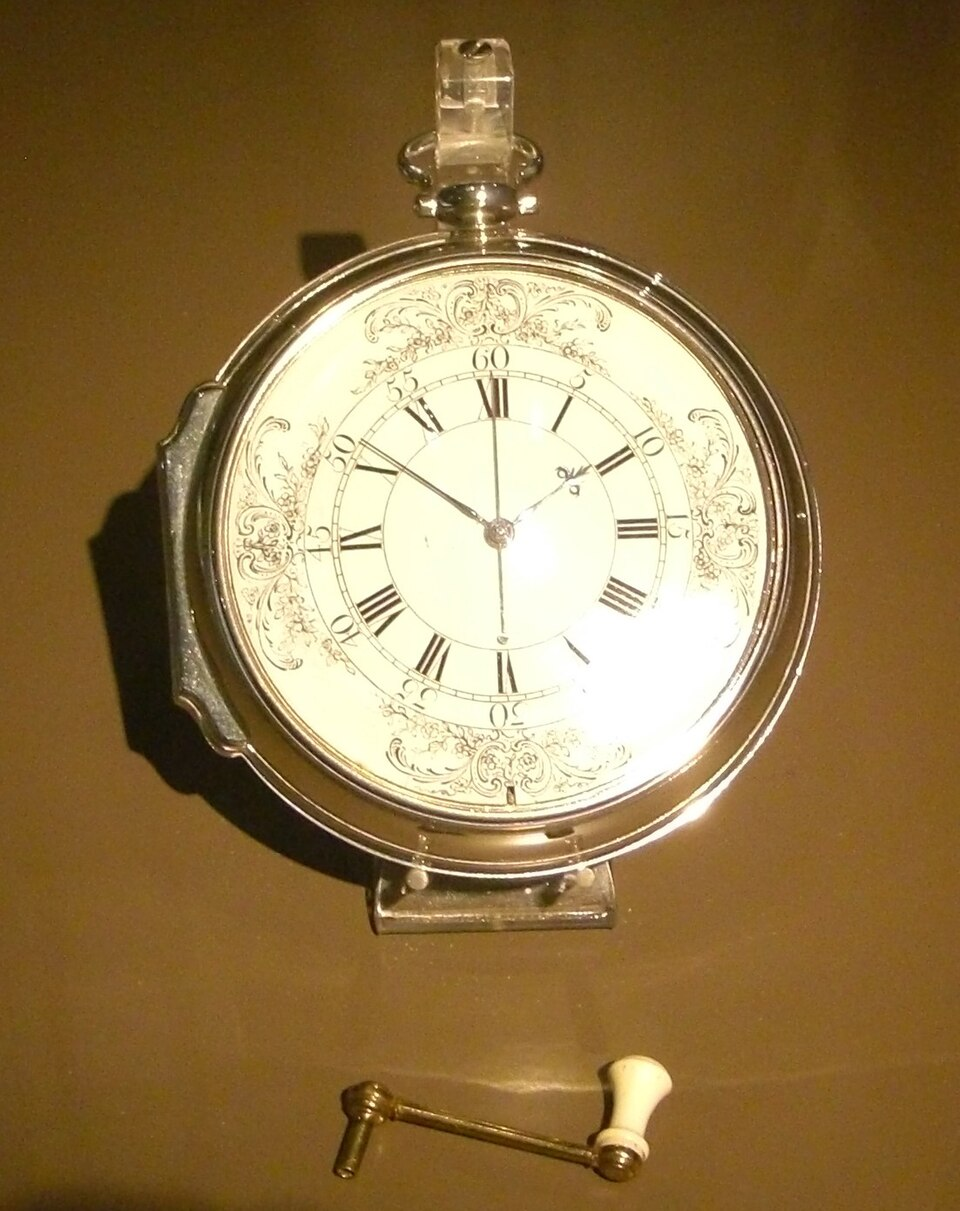
\includegraphics[width=\linewidth]{images/book1/g6-harrison-h4.jpg}\\[2pt]
{\footnotesize हैरिसन की H4, राष्ट्रीय समुद्री संग्रहालय, ग्रीनविच। (फ़ोटो:
कर्नल वार्डेन, CC BY-SA 3.0, विकिमीडिया कॉमन्स के ज़रिए।)}
% ledger: commons:harrison-h4
\end{minipage}
\end{history}

\section{अभ्यास}

\begin{exercise}[$\star$]\label{exo:g6:latitude-longitude:1}
उतारो और पूरा करो: ``\omterm{def:g6:latitude-longitude:latitude}{अक्षांश} \ldots{} से नापा जाता है और
$0^\circ$ से \ldots{} तक जाता है; \omterm{def:g6:latitude-longitude:longitude}{देशांतर} \ldots{} \omterm{def:g6:latitude-longitude:longitude}{याम्योत्तर} से नापा जाता है और
$0^\circ$ से \ldots{} तक जाता है।''
\end{exercise}

\begin{exercise}[$\star$]\label{exo:g6:latitude-longitude:2}
\omterm{def:g3:continents-and-oceans:poles}{उत्तरी ध्रुव} का \omterm{def:g6:latitude-longitude:latitude}{अक्षांश} क्या है? \omterm{def:g3:continents-and-oceans:poles}{दक्षिणी ध्रुव} का? \omterm{def:g3:continents-and-oceans:equator}{भूमध्य रेखा} पर के किसी
शहर का?
\end{exercise}

\begin{exercise}[$\star$]\label{exo:g6:latitude-longitude:3}
तेरह शहरों वाले \omterm{def:g2:drawing-to-map:map}{मानचित्र} की मदद से बताओ कि इनमें से हर शहर किस \omterm{def:g3:continents-and-oceans:equator}{गोलार्ध} में है, उत्तरी
या दक्षिणी, और \omterm{def:g6:latitude-longitude:longitude}{प्रमुख याम्योत्तर} की किस ओर, पूर्व या पश्चिम: सिडनी, न्यूयॉर्क,
काहिरा, रियो डी जनेरो।
\end{exercise}

\begin{exercise}[$\star$]\label{exo:g6:latitude-longitude:4}
सही या ग़लत? ग़लत वाक्यों को सुधारो।
(क) सभी \omterm{def:g6:latitude-longitude:longitude}{याम्योत्तर} \omterm{def:g3:continents-and-oceans:poles}{ध्रुवों} पर मिलते हैं।
(ख) सभी \omterm{def:g6:latitude-longitude:latitude}{अक्षांश रेखाओं} की लंबाई बराबर है।
(ग) \omterm{def:g3:continents-and-oceans:equator}{भूमध्य रेखा} एक \omterm{def:g6:latitude-longitude:latitude}{अक्षांश रेखा} है।
(घ) \omterm{def:g6:latitude-longitude:longitude}{प्रमुख याम्योत्तर} पेरिस से होकर जाता है।
\end{exercise}

\begin{exercise}[$\star\star$]\label{exo:g6:latitude-longitude:5}
तेरह शहरों वाले \omterm{def:g2:drawing-to-map:map}{मानचित्र} की मदद से बताओ: कौन-सा शहर लगभग
$30^\circ$\,उ, $31^\circ$\,पू पर है? कौन-सा लगभग $41^\circ$\,उ,
$74^\circ$\,प पर? टोक्यो के अनुमानित निर्देशांक बताओ।
% ledger: data:b1-ne-places (cities.py main table)
\end{exercise}

\begin{exercise}[$\star\star$]\label{exo:g6:latitude-longitude:6}
शहर~A \omterm{def:g6:latitude-longitude:longitude}{देशांतर} $0^\circ$ पर है और शहर~B \omterm{def:g6:latitude-longitude:longitude}{देशांतर} $45^\circ$\,पू पर।
उनकी दोपहरों में कितने घंटे का अंतर है? किस शहर में दोपहर पहले होती है?
\end{exercise}

\begin{exercise}[$\star\star$]\label{exo:g6:latitude-longitude:7}
मुंबई लगभग $73^\circ$\,पू पर है। उसका आदर्श \omterm{def:g6:latitude-longitude:time-zone}{समय-क्षेत्र} निकालो। जब ग्रीनविच में
दोपहर हो, तब आदर्श क्षेत्रों में मुंबई में क्या समय होगा?
% ledger: data:b1-ne-places (cities.py: 72.88 E, zone +5)
\end{exercise}

\begin{exercise}[$\star\star$]\label{exo:g6:latitude-longitude:8}
\omterm{def:g6:latitude-longitude:latitude}{अक्षांश} का हर अंश लगभग \qty{111}{km} का होता है। $30^\circ$\,उ पर का कोई शहर अपने
\omterm{def:g6:latitude-longitude:longitude}{याम्योत्तर} के साथ नापने पर \omterm{def:g3:continents-and-oceans:equator}{भूमध्य रेखा} से कितनी दूर है? \omterm{def:g3:continents-and-oceans:poles}{उत्तरी ध्रुव} \omterm{def:g3:continents-and-oceans:equator}{भूमध्य रेखा} से
कितनी दूर है?
% ledger: rmg:latitude-def
\end{exercise}

\begin{exercise}[$\star\star$]\label{exo:g6:latitude-longitude:9}
न्यूयॉर्क क्षेत्र $-5$ में है और टोक्यो क्षेत्र $+9$ में। उनकी घड़ियों में कितने घंटे
का अंतर है? जब न्यूयॉर्क में सोमवार सुबह के 8~बजे हों, तब टोक्यो में क्या समय
और कौन-सा दिन होगा?
% ledger: data:b1-ne-places (cities.py: zones -5 and +9)
\end{exercise}

\begin{exercise}[$\star\star$]\label{exo:g6:latitude-longitude:10}
लीना कहती है: ``सूर्य पूर्व में उगता है, इसलिए पूर्व के शहर पश्चिम के शहरों से पहले
सूर्य को उगते देखते हैं।'' क्या वह सही है? पृथ्वी के घूमने से
समझाओ।
\end{exercise}

\begin{exercise}[$\star\star\star$]\label{exo:g6:latitude-longitude:11}
एक जहाज़ की घड़ी दिन में 3~सेकंड आगे हो जाती है (वह बहुत तेज़ चलती है)। (क) 42~दिन
की यात्रा के बाद वह कितने सेकंड आगे होगी? (ख) पृथ्वी 4~मिनट में, यानी 240~सेकंड
में, एक अंश घूमती है। घड़ी की ग़लती \omterm{def:g6:latitude-longitude:longitude}{देशांतर} में कितने अंश की ग़लती
बनाती है? (ग) \omterm{def:g3:continents-and-oceans:equator}{भूमध्य रेखा} पर \omterm{def:g6:latitude-longitude:longitude}{देशांतर} का एक अंश लगभग \qty{111}{km} का होता है।
\omterm{def:g3:continents-and-oceans:equator}{भूमध्य रेखा} पर नाविक लगभग कितने किलोमीटर
ग़लत होगा?
% ledger: rmg:longitude-act-1714, rmg:15deg-per-hour, rmg:latitude-def
\end{exercise}

\begin{exercise}[$\star\star\star$]\label{exo:g6:latitude-longitude:12}
एक हवाई जहाज़ सोमवार शाम 6~बजे टोक्यो (क्षेत्र $+9$) से चलता है और प्रशांत के पार पूर्व
की ओर लॉस एंजेलिस (क्षेत्र $-8$) तक उड़ता है। उड़ान 10~घंटे की है। (क) जहाज़ के
चलते समय ग्रीनविच में क्या समय है? (ख) उसके उतरते समय
ग्रीनविच में क्या समय है? (ग) उसके उतरते समय लॉस
एंजेलिस में स्थानीय समय और दिन क्या है? यात्री क्यों कहते हैं कि इस उड़ान में ``तुम
उड़ने से पहले ही उतर जाते हो''?
\end{exercise}

\section{समस्या: दुनिया भर में एक वीडियो कॉल}

\begin{problem}[{सप्ताहांत समस्या --- पाँच दोस्त, चार समय-क्षेत्र और एक
तिथि रेखा: कॉल शुरू होते समय ऑकलैंड में क्या समय है?}]
\label{pb:g6:latitude-longitude:1}
% ledger: data:b1-ne-places, rmg:15deg-per-hour, planet:Earth.day (cities.py, time_zones.py; test_cities_zones_used_in_the_problem)
लीना लंदन में रहती है। वह छुट्टियों में मिले चार दोस्तों के साथ एक वीडियो कॉल रखना
चाहती है: रियो डी जनेरो में एना, टोक्यो में केंजी, ऑकलैंड में मिया
और लॉस एंजेलिस में सैम। इस समस्या में हम आदर्श \omterm{def:g6:latitude-longitude:time-zone}{समय-क्षेत्रों} का प्रयोग करते हैं।

\begin{center}
\small
\begin{tabular}{lll}
\hline
दोस्त & शहर & निर्देशांक\\
\hline
लीना & लंदन & $52^\circ$\,उ, $0^\circ$\\
एना & रियो डी जनेरो & $23^\circ$\,द, $43^\circ$\,प\\
केंजी & टोक्यो & $36^\circ$\,उ, $140^\circ$\,पू\\
मिया & ऑकलैंड & $37^\circ$\,द, $175^\circ$\,पू\\
सैम & लॉस एंजेलिस & $34^\circ$\,उ, $118^\circ$\,प\\
\hline
\end{tabular}
\end{center}

\medskip
\noindent\textbf{भाग I --- दोस्त कहाँ रहते हैं।}
\begin{enumerate}
  \item कौन-से दोस्त \omterm{def:g3:continents-and-oceans:equator}{दक्षिणी गोलार्ध} में रहते हैं?
  \item कौन-से दोस्त \omterm{def:g6:latitude-longitude:longitude}{प्रमुख याम्योत्तर} के पश्चिम में रहते हैं?
  \item कौन-सा दोस्त \omterm{def:g3:continents-and-oceans:equator}{भूमध्य रेखा} से सबसे दूर रहता है?
  \item कौन-सा दोस्त $180^\circ$ \omterm{def:g6:latitude-longitude:longitude}{याम्योत्तर} के सबसे पास रहता है? उससे \omterm{def:g6:latitude-longitude:longitude}{देशांतर} के
        कितने अंश दूर?
\end{enumerate}

\medskip
\noindent\textbf{भाग II --- क्या समय है?}
\begin{enumerate}[resume]
  \item पृथ्वी एक घंटे में कितने अंश घूमती है?
  \item हर दोस्त के शहर का आदर्श \omterm{def:g6:latitude-longitude:time-zone}{समय-क्षेत्र} निकालो।
  \item लीना शुक्रवार को लंदन के समय से रात 8~बजे कॉल शुरू करने का प्रस्ताव रखती है।
        तब रियो डी जनेरो में क्या समय और कौन-सा दिन होगा? टोक्यो में?
  \item केंजी जवाब देता है कि वह तब सो रहा होगा। समझाओ कि टोक्यो में पहले से ही
        शनिवार क्यों है।
\end{enumerate}

\medskip
\noindent\textbf{भाग III --- तिथि रेखा पार करना।}
\begin{enumerate}[resume]
  \item कॉल शुरू होते समय लॉस एंजेलिस में क्या समय और कौन-सा दिन है?
  \item ऑकलैंड की घड़ियाँ लॉस एंजेलिस से कितने घंटे आगे हैं?
  \item ऑकलैंड से लॉस एंजेलिस की ओर पूर्व में चलता एक जहाज़ \omterm{def:g6:latitude-longitude:date-line}{तिथि रेखा} पार करता है।
        क्या वह अगले दिन में आगे जाता है या पिछले दिन में लौटता है?
  \item कॉल शुरू होते समय ऑकलैंड में स्थानीय समय और दिन क्या है?
\end{enumerate}
\end{problem}
